%%% Local Variables:
%%% TeX-master: "poster"
%%% End:

\begin{minipage}[t]{0.49\linewidth}
  The synthesis objective is to shape the norm of two filters \(H_1(s)\) and \(H_2(s)\) while ensuring their complementary property.
  This is equivalent as to finding stable transfer functions \(H_1(s)\) and \(H_2(s)\) such that conditions \eqref{eq:comp_filter_problem_form} are satisfied.
  \[ \left\{
      \begin{array}{ll}
        H_1(s) + H_2(s) = 1 \\
        |H_1(j\omega)| \le \frac{1}{|W_1(j\omega)|} \quad \forall\omega \\
        |H_2(j\omega)| \le \frac{1}{|W_2(j\omega)|} \quad \forall\omega
      \end{array}
    \right.  \]

  \begin{tikzfigure}[Architecture used for $\mathcal{H}_\infty$ synthesis]
    \label{fig:h_infinity_robust_fusion}
    \centering
    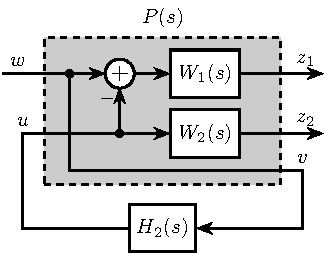
\includegraphics[scale=1.8]{figs/h_infinity_robust_fusion.pdf}
  \end{tikzfigure}

\end{minipage}\hfill
\begin{minipage}[t]{0.49\linewidth}
  \begin{tikzfigure}[Frequency response of the weighting functions and complementary filters obtained using $\mathcal{H}_\infty$ synthesis]
    \label{fig:hinf_synthesis_results}
    \centering
    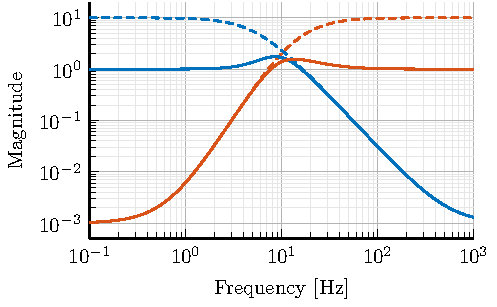
\includegraphics[scale=1.8]{figs/hinf_synthesis_results.pdf}
  \end{tikzfigure}
\end{minipage}

\textbf{Weighting Function Design}

\begin{minipage}[t]{0.49\linewidth}
  \begin{equation*}
    W(s) = \left( \frac{
        \hfill{} \frac{1}{\omega_0} \sqrt{\frac{1 - \left(\frac{G_0}{G_c}\right)^{\frac{2}{n}}}{1 - \left(\frac{G_c}{G_\infty}\right)^{\frac{2}{n}}}} s + \left(\frac{G_0}{G_c}\right)^{\frac{1}{n}}
      }{
        \left(\frac{1}{G_\infty}\right)^{\frac{1}{n}} \frac{1}{\omega_0} \sqrt{\frac{1 - \left(\frac{G_0}{G_c}\right)^{\frac{2}{n}}}{1 - \left(\frac{G_c}{G_\infty}\right)^{\frac{2}{n}}}} s + \left(\frac{1}{G_c}\right)^{\frac{1}{n}}
      }\right)^n
  \end{equation*}
\end{minipage}\hfill
\begin{minipage}[t]{0.49\linewidth}
  \begin{tikzfigure}[Magnitude of a weighting function generated using the proposed formula \eqref{eq:weight_formula}, $G_0 = 1e^{-3}$, $G_\infty = 10$, $\omega_c = \SI{10}{Hz}$, $G_c = 2$, $n = 3$]
    \label{fig:weight_formula}
    \centering
    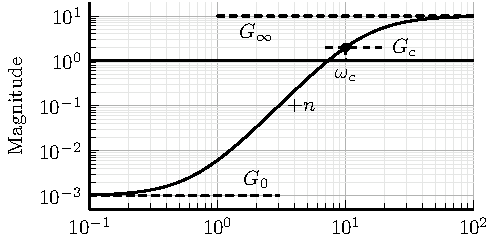
\includegraphics[scale=1.8]{figs/weight_formula.pdf}
  \end{tikzfigure}
\end{minipage}

% \textbf{Three Complementary Filters}

% \begin{minipage}[t]{0.49\linewidth}
%   \begin{tikzfigure}[Architecture for $\mathcal{H}_\infty$ synthesis of three complementary filters]
%     \label{fig:comp_filter_three_hinf}
%     \centering
%     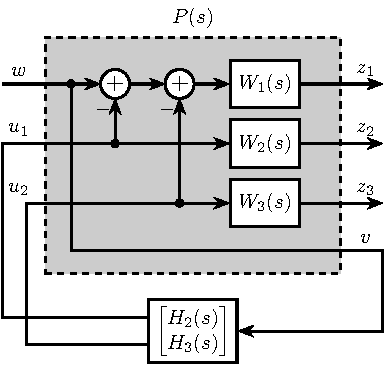
\includegraphics[scale=1.8]{figs/comp_filter_three_hinf.pdf}
%   \end{tikzfigure}
% \end{minipage}\hfill
% \begin{minipage}[t]{0.49\linewidth}
%   \begin{tikzfigure}[Frequency response of the weighting functions and three complementary filters obtained using $\mathcal{H}_\infty$ synthesis]
%     \label{fig:hinf_three_synthesis_results}
%     \centering
%     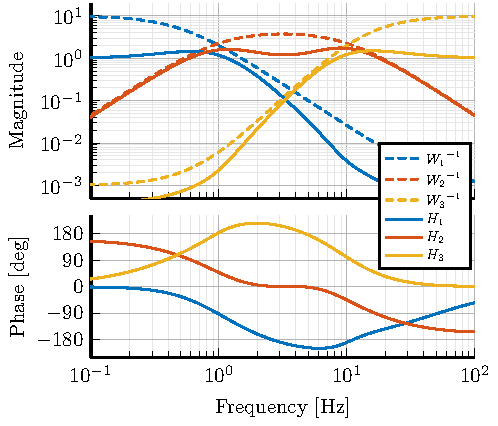
\includegraphics[scale=1.8]{figs/hinf_three_synthesis_results.pdf}
%   \end{tikzfigure}
% \end{minipage}
